\section{Passerine: An Agent-based Repair System}
\label{sec:passerine}


To establish a repair performance floor for agent-based APR on GITS-Eval, we developed an APR agent, Passerine, inspired by SWE-Agent.
Like SWE-Agent, Passerine uses a ReAct~\cite{react} loop to iteratively produce ``thoughts,'' run commands against the current state of the workspace, and observe the commands' results; the output of the agent is a modified workspace in which, if the agent is successful, the bug is fixed, as well as a trace of the agent's execution, for human interpretation and debugging.
Similarly to SWE-Agent, we expose commands to the agent that are suited both to the APR task and designed with the ergonomics of the ``agent-computer interface'' in mind; these commands include both workalikes of the SWE-Agent commands (file viewing, file editing, and terminating the agent), as well as commands that provide functionality specific to Google's development environment (compiling and running tests, searching the index of Google's monorepo).

\emph{Unlike} SWE-Agent, we find that we do not need to expose a full Linux command line to the agent, e.g., via containerization.
Google's test-running infrastructure already provides sufficient containerization~\cite{potvingoogle}. Our experience, as well as prior work in agent-based APR like RepairAgent~\cite{repairagent} and AutoCodeRover~\cite{autocoderover}, shows that a small, APR-focused command set is sufficient for bug-fixing.

Passerine is intentionally simple and minimal, avoiding complex architecture or explicitly dividing the APR process into discrete phases like localization, editing, testing, and so forth.
This simple approach is validated by the effectiveness of agents without prespecified control flow like SWE-Agent~\cite{sweagent}, CodeAct~\cite{codeact}, and OpenDevin~\cite{opendevin}.
We show, through the first evaluation of a simple SWE-Agent-like APR system in an industrial setting, that, in spite of its minimalism, our agent is capable of addressing many real-world bugs.










\subsection{Agent Design}

Passerine is a fully ``dynamic'' agent in the sense that it has no prespecified control flow. Every step in Passerine corresponds to a ReAct~\cite{react} style step, depicted
in Figure~\ref{fig:passerine-high-level-react},
where the agent issues an LLM prompt asking for the next command to perform and obtains back a response in the form of “thought” and “action.” The thought is a natural language fragment reasoning about the state of the agent and describing the next step. The action is a code fragment consisting of a Unix-like tool name, associated arguments for its call, and, for some commands (e.g., text editing), multiline input text. The agent framework then parses that command, executes it,
and replies to the agent with any observable outcomes.




\begin{figure}
    \centering
    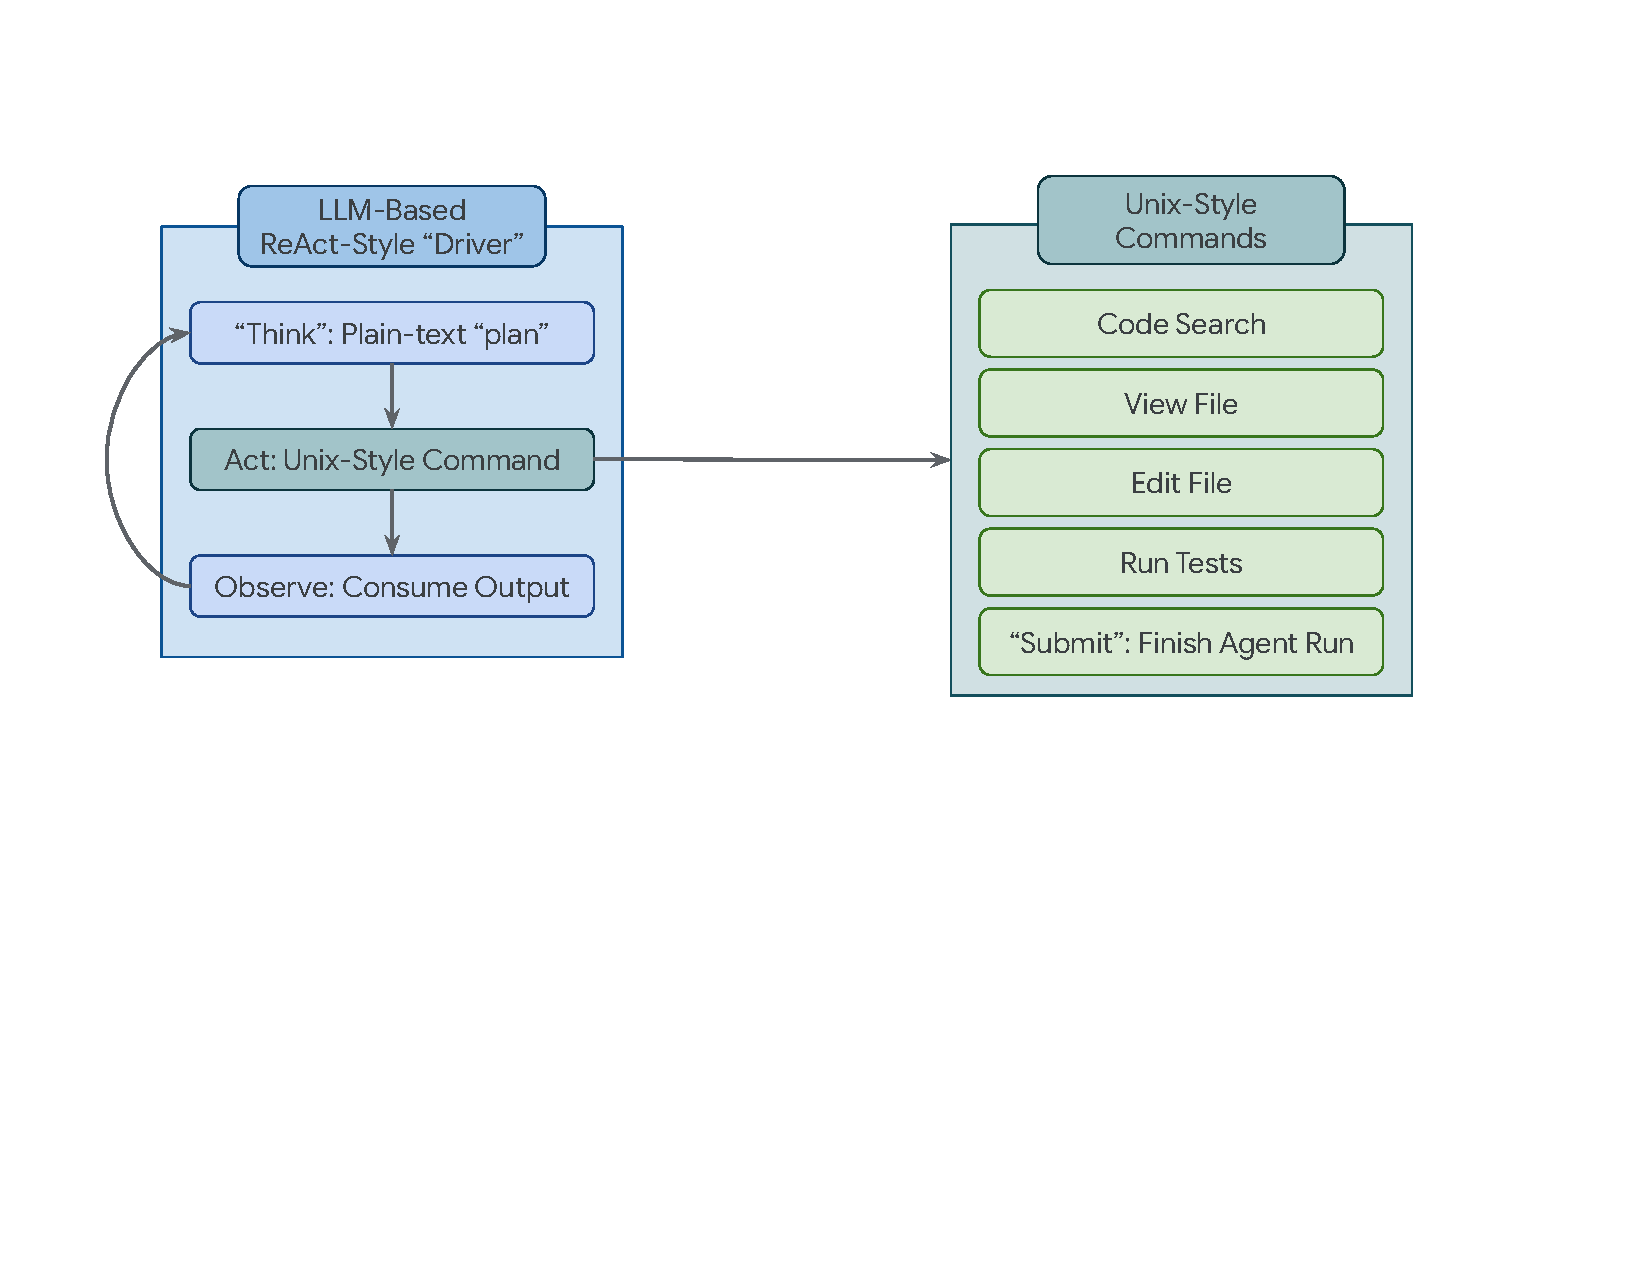
\includegraphics[width=\columnwidth]{figures/passerine-high-level-overview.pdf}
    \caption{A high-level overview of Passerine’s ReAct-style dynamic loop and the Unix-style (adapted to Google) commands exposed as tools for the agent to use.
    }
    \label{fig:passerine-high-level-react}
\end{figure}


\cheapsubsection{LLM Prompting and History:} When querying the LLM to obtain a new step, the agent includes information on the current state of the environment. Currently, 
Passerine includes the entire history of the agent. This has the benefit of simplicity and is facilitated by longer-context models. However, as we describe in Section~\ref{sec:challenges}, we can still encounter agent runs that exceed LLM context limits and thus we could benefit from more-sophisticated history management strategies.

\cheapsubsection{Agent Termination:} Passerine can call a \lstinline!finish [success|failure]! command to terminate, along
with the agent's judgment of the outcome.
To avoid non-termination, we also enforce a maximum step limit.


\cheapsubsection{Isolation:} Because the agent makes stateful changes to the environment, we rely 
on Google's codebase containerization~\cite{potvingoogle} to enforce isolation between different agent executions. We describe more of the infrastructure associated with running the agent in Section~\ref{sec:evaluation-framework}.

\subsection{Commands}\label{sec:commands}
Passerine takes a minimalist approach by providing a set of only 5
commands (and 1 additional alias commonly referenced in bug descriptions) that the agent can use, which are designed to interact with
Google internal APIs. A direct benefit of using a limited command set, restricted only to a few operations that can be implemented on top of already-containerized APIs,
is that Passerine \emph{does not} require a full virtual machine for isolation, improving scalability.


Commands in our design have a uniform input and output interface. For inputs, commands accept zero or more positional arguments, followed by arbitrary text fragments after a newline (e.g. to support editing). Every command output consists of an exit code and output text. The output text is the observable behavior that is exposed to the agent in its history.


We now briefly describe each command shown on the right-hand side of Figure~\ref{fig:passerine-high-level-react}.

\begin{itemize}
    \item \textbf{cat:} Takes a single file in the workspace and lists its contents using internal APIs. Every line is prefixed with a line number.
    
    \item \textbf{code\_search}: Takes one or more terms and concatenates these to issue a query for the Google internal Code Search API~\cite{sadowski2015developers}.
    
    
    \item \textbf{edit:} Takes a filename, starting and ending lines, and the replacement text with which to substitute the identified line region. When the edit is applied, the command's output text corresponds to the modified content (along with up to 3 context lines around it), where lines have been prefixed with the resulting line numbering post-edit. Edits are done through an internal API, which interacts with the isolated codebase container.

    \item \textbf{bazel}: Takes a test suite target, along with arbitrary parameters for test suite execution, and issues a distributed build/execution~\cite{greenberg2016building} for the associated target  using Google's internal build tool Bazel~\cite{wang2021smart}. The framework then parses the build report, extracts outcomes and relevant log excerpts, and surfaces these as an observable output for the agent.
    
    
    \item \textbf{finish}: Takes as argument 
    ``\lstinline|success|'' or ``\lstinline|failure|''
    and terminates agent execution.

\end{itemize}

All commands are implemented as simple Python functions, which easily support incorporating command validation and logging logic. We present each command to Passerine in its
initial prompt, providing a high-level description of the behavior, along with
fixed basic examples showing how each command can be used. To illustrate, Figure~\ref{fig:prompt-skeleton} shows our agent's system prompt template, along with a command doc template which is populated by each command's implementation.



\begin{figure}[h]
\vspace{-0.0cm}
    \centering
\begin{adjustbox}{width=0.49\textwidth}
\begin{tabular}{c}
\toprule
\footnotesize{System prompt template}\\
\midrule
\begin{minipage}[t]{0.45\textwidth}\vspace{-1em}
\begin{lstlisting}[escapeinside=||, breaklines]{text}
SETTING: You are a software engineer working on fixing bugs.

You are only allowed to use the following commands:

COMMANDS:
LIST_OF_COMMAND_DOCS

Output instructions:
1. Your output should always include only one thought section and one action.
2. Explain what you are doing in the thought section.
3. An action should be a single command from the COMMANDS section.
4. Do not include more than one command in the action.

Here is an example output:
THOUGHT:
First I'll start by running the test to reproduce the issue.
ACTION:
```tool_code
bazel test //some/target
```
\end{lstlisting}
\end{minipage}\\
\midrule
\footnotesize{Command doc template}\\
\midrule
\begin{minipage}[t]{0.45\textwidth}\vspace{-1em}
\begin{lstlisting}[escapeinside=||, breaklines]{text}
Command name: COMMAND_NAME
# COMMAND_NAME
## Description:
DESCRIPTION_TEXT
## Usage:
USAGE_TEXT
## Examples:
EXAMPLE_TEXT
\end{lstlisting}
\end{minipage}\\
\bottomrule
\end{tabular}
\end{adjustbox}
\vspace{-0.0cm}
\caption{System and command documentation template for Passerine}
\vspace{-0.0cm}
\label{fig:prompt-skeleton}
\end{figure}

\subsection{Evaluation Framework for Historic Bugs}\label{sec:evaluation-framework}


As part of developing Passerine, we also implement a framework which allows us to evaluate different agent configurations on Google infrastructure and analyze their performance, all in the context of historical bugs that have already fixed.




\cheapsubsection{Setup:} Before evaluating an agent, the framework sets up the environment by 1) loading the appropriate bug information and 2) checking out the repository state (also known as a changelist, which is the snapshot that undergoes code review\footnote{Google engineering practices documentation: \url{https://github.com/google/eng-practices}}) \emph{prior} to the associated ground-truth fix. Then
the framework reproduces the bug in this environment, to confirm that the setup correctly exposes the issue as expected. To do so, our framework allows benchmark repair tasks to specify the expected test targets to run and any files that are relevant to that state, and may need to be copied over from the ground-truth patch.
In practice, for machine-reported bugs, our framework automatically extracts bug-reproducing tests from the associated issue content using regular expressions.
Note that, for TOD tests, the associated test specifies a \emph{single} ordering of the test cases which exhibits the order dependency.
For human-reported bugs,
our framework has an offline pass that uses Google
tooling to identify test targets that depend on the test
files modified by the patch, considers these as candidate 
bug reproducing tests, and prunes the set down to those
that fail before and pass after the ground-truth patch has
been applied.

After the bug has been confirmed, the framework reverts the repository state to reflect only information available before the ground-truth fix was produced.


\cheapsubsection{Execution:} During execution, the agent operates independently, but the framework records agent-related events into a structured log for offline analysis. Logs reflect events such as commands issued by the agent and outputs obtained from the environment, as well as information such as what files/lines have entered the agent history (for localization analysis).
Importantly, our evaluation framework ensures, that during
command execution, there is no data leakage from future
states in the repository, e.g. code search results
are limited to those up to the commit preceding the ground-truth fix.

\cheapsubsection{Cleanup:}
After the agent has finished its execution (either through step budget exhaustion or issuing a finish command), the framework once again patches in any necessary test files and executes the bug reproduction test targets to confirm that the agent’s changes to the repository state result in a successful execution. 

(Note that \emph{specifically} the ground-truth test file is used to evaluate the plausibility of agent fixes for human-reported bugs; also, we do not evaluate agent modifications to test files, leaving this to future work.)

At this point, the framework also records structured logs of the execution, as well as evaluation reproduction information.
